\documentclass[11pt]{article}
\usepackage{float} % floating shapes and tables
\usepackage{graphicx}
\usepackage{amssymb} % math symbols (Real Set)
\usepackage{physics} % all of those bras and kets
\usepackage[hidelinks]{hyperref} % links

\title{$SU(2)$ gate composition}
\author{S. S. Kahani}
\date{April 27, 2019}
\begin{document}

\maketitle

\section{Introduction}
we can represent each $SU(2)$ elements in terms of \cite{hamada}
\begin{equation}
 u(\theta, \vu{n}) = e^{i\theta \vu{n} \cdot \va*{\sigma}}
\end{equation}

where 

\[ \sigma_1 = \begin{pmatrix} 0 & 1 \\ 1 & 0 \end{pmatrix}, \sigma_2 = \begin{pmatrix} 0 & -i \\ i & 0 \end{pmatrix}, \sigma_3 = \begin{pmatrix} 1 & 0 \\ 0 & -1 \end{pmatrix} \]

and therefore $\vu{n}$ is a 3-D unit vector.

the pair of $(\theta, \vu{n})$ can be a vector in 3-D space with magnitude of $\theta$ (which is bounded) and orientation of $\vu{n}$.%
%
\footnote{A $SU(2)$ matrix can be represented with multiple $(\theta, \vu{n})$ pairs, but one and only one of them satifies $0 \le \theta \le \pi$.}

\section{Description}

\subsection{extraction of vector representation}
for an arbitrary unitary matrix $u$ we have

\[ u = \begin{pmatrix} a & b \\ c & d \end{pmatrix} \]
 
on the other hand
 
\[ u = e^{i\theta \vu{n} \cdot \va*{\sigma}} = I \cos\theta + i \vu{n} \cdot \va*{\sigma} \sin\theta \]

where $I$ is a $2\times 2$ identity matrix

\begin{gather*}
u = e^{i\theta \vu{n} \cdot \va*{\sigma}} = I \cos\theta + i n_1 \sigma_1 \sin\theta + i n_2 \sigma_2 \sin\theta  + i n_3 \sigma_3 \sin\theta \\
\begin{align*} u =& \begin{pmatrix}
\cos\theta & 0 \\ 
0 & \cos\theta 
\end{pmatrix} + 
\begin{pmatrix} 
0 & in_1\sin\theta \\
in_1\sin\theta & 0 
\end{pmatrix} + \\ &
\begin{pmatrix} 
0 & n_2\sin\theta \\
-n_2\sin\theta & 0 
\end{pmatrix} +
\begin{pmatrix} 
in_3\sin\theta & 0\\
0 & -in_3\sin\theta 
\end{pmatrix}
\end{align*} \\
u = \begin{pmatrix}
\cos\theta + in_3\sin\theta & n_2\sin\theta + i n_1\sin\theta \\ 
- n_2\sin\theta + i n_1\sin\theta & \cos\theta - in_3\sin\theta
\end{pmatrix}
\end{gather*}

now, formula below shows how to extract $(\theta, \vu{n})$ from matrix elements

\begin{equation}
\begin{cases}
  \theta = \arccos (a + d) \\
  n_1 = \frac{b + c}{2i\sin\theta} \\
  n_2 = \frac{b - c}{2\sin\theta} \\
  n_3 = \frac{a - d}{2i\sin\theta} \\
\end{cases}
\end{equation}

\subsection{state visualization}

assuming two unitary matrices
\[ u_1 = \frac{1}{\sqrt{2}} \begin{pmatrix} 1 & 1 \\ 1 & -1 \end{pmatrix} \text{a.k.a. Hadamard}, u_2 = \begin{pmatrix} 1 & 0 \\ 0 & e^{i\frac{\pi}{4}} \end{pmatrix} \text{a.k.a. T-Gate}  \]

by ignoring their phase, we have
\[ \hat{u_i} = \frac{1}{\sqrt{\det u_i}} u_i, \hat{u_i} \in SU(2) \]
we define
\[ S_1 = \{\hat{u_1}, \hat{u_2}\}, S_n = \{x y | x \in S_{n-1}, y \in S_{1}\} \]

\begin{figure}[H]
\centering
\includegraphics[width=0.3\textwidth]{level_19.png}
\includegraphics[width=0.3\textwidth]{level_19_rotated.png}
\includegraphics[width=0.3\textwidth]{level_12.png}
\caption{from left to right: $\bigcap_{i=0}^{19} S_i$ ,\newline $\bigcap_{i=0}^{19} S_i$ rotated, $\bigcap_{i=0}^{12} S_i$  }
\end{figure}

\subsection{gate errors in $SU(2)$}

as we defined error for an operator $e$ as an estimation of $u$
\[ \varepsilon(e, u) = \max_{\ket{v}} || (e - u) \ket{v} || \]

then 
\[ \varepsilon = \max_{\ket{v}} \bra{v}(e - u)^\dagger (e - u) \ket{v} \]
\[ \varepsilon = 2 - \min_{\ket{v}} \bra{v} (e^\dagger u + u^\dagger e) \ket{v} \]

now by replacing each $SU(2)$ matrix we have

\begin{multline*}
\varepsilon = 2 - \min_{\ket{v}} 
\bra{v} \Big(
(I \cos\theta_e + i \vu{n}_e \cdot \va*{\sigma} \sin\theta_e)^\dagger
(I \cos\theta_u + i \vu{n}_u \cdot \va*{\sigma} \sin\theta_u) - \\
(I \cos\theta_u + i \vu{n}_u \cdot \va*{\sigma} \sin\theta_u)^\dagger
(I \cos\theta_e + i \vu{n}_e \cdot \va*{\sigma} \sin\theta_e)
\Big) \ket{v}
\end{multline*}

knowing $\sigma_i = \sigma_i^\dagger$

\begin{gather*}
\begin{align*}
\varepsilon = 2 - \min_{\ket{v}} \bra{v} \Big( &
2 I \cos\theta_e\cos\theta_u + \\ &
\big(
(\vu{n}_u \cdot \va*{\sigma}) (\vu{n}_e \cdot \va*{\sigma}) +
(\vu{n}_e \cdot \va*{\sigma}) (\vu{n}_u \cdot \va*{\sigma})\big) \sin\theta_u\sin\theta_e + \\ 
& i(\vu{n}_u \cdot \va*{\sigma})\cos\theta_e\sin\theta_u  -
i(\vu{n}_e \cdot \va*{\sigma})\cos\theta_u\sin\theta_e + \\
& i(\vu{n}_e \cdot \va*{\sigma})\cos\theta_u\sin\theta_e  -
i(\vu{n}_u \cdot \va*{\sigma})\cos\theta_e\sin\theta_u
\Big) \ket{v}
\end{align*} \\
\begin{align*}
\varepsilon = 2 - \min_{\ket{v}} \bra{v} \Big(
2 I \cos\theta_e\cos\theta_u + 
\big(
(\vu{n}_u \cdot \va*{\sigma}) (\vu{n}_e \cdot \va*{\sigma}) +
(\vu{n}_e \cdot \va*{\sigma}) (\vu{n}_u \cdot \va*{\sigma})\big) \sin\theta_u\sin\theta_e \Big) \ket{v}
\end{align*} \\
\begin{align*}
\varepsilon = 2 - 2 \cos\theta_e \cos\theta_u - \sin\theta_u\sin\theta_e \min_{\ket{v}} \bra{v} \Big(
(\vu{n}_u \cdot \va*{\sigma}) (\vu{n}_e \cdot \va*{\sigma}) +
(\vu{n}_e \cdot \va*{\sigma}) (\vu{n}_u \cdot \va*{\sigma})\Big) \ket{v}
\end{align*} \\
\begin{align*}
\varepsilon = 2 - 2 \cos\theta_e \cos\theta_u - \sin\theta_u\sin\theta_e \min_{\ket{v}} \bra{v} \Big( (\sum_i n_{Ui} \sigma_i) (\sum_i n_{Ei} \sigma_i) + (\sum_i n_{Ei} \sigma_i) (\sum_i n_{Ui} \sigma_i) \Big) \ket{v}
\end{align*} \\
\begin{align*}
\varepsilon = 2 - 2 \cos\theta_e \cos\theta_u - \sin\theta_u\sin\theta_e \min_{\ket{v}} \bra{v} \Big(2\sum_i n_{Ui}n_{Ei} I + & i\sum_{i,j,k} n_{Ui} n_{Ej} \epsilon_{ijk}  \sigma_k \\ - & i\sum_{i,j,k} n_{Ei} n_{Uj} \epsilon_{ijk} \sigma_k \Big) \ket{v}
\end{align*} \\
\end{gather*}

finally,
\begin{equation}
\varepsilon = 2 - 2 \cos\theta_e \cos\theta_u - 2\sin\theta_u\sin\theta_e (\vu{n}_u\cdot \vu{n}_e)
\end{equation}

\subsection{Solovay-Kitaev theorem for $SU(2)$}

for an arbitrary unitary matrix $u$, minimum error of approximation with $n$ gates will be
\[ \varepsilon^*(e, n) = \min_{e \in S_n} \varepsilon(e, u) \]

in the way of proofing Solovay-Kitaev theorem is shown that \cite{ozlos} 

\begin{gather*}
\text{if } \varepsilon^*(e, n_0) \le \varepsilon_0 \rightarrow \exists s, ~ \forall k: ~
\varepsilon^*(e, \sum_{m=0}^k 5^m n_0) \le \frac{(s\varepsilon_0)^{(1.5^k)}}{s} \\
%
\text{if } \varepsilon^*(e, n_0) \le \varepsilon_0 \rightarrow \exists s, ~ \forall k: ~
\varepsilon^*(e, \frac{5}{4} 5^k n_0) \le \frac{(s\varepsilon_0)^{(1.5^k)}}{s} \\
%
\text{if } \varepsilon^*(e, n_0) \le \varepsilon_0 \rightarrow \exists s,
\varepsilon^*(e, \alpha n_0) \le \frac{(s\varepsilon_0)^{(\alpha^{\log 1.5/ \log 5})}}{s} \\
%
\text{if } \log\varepsilon^*(e, n_0) \le \delta_0 \rightarrow \exists s,
\log\varepsilon^*(e, \alpha n_0) \le (\alpha^{\log 1.5/ \log 5}) (\log s + \delta_0) - \log s
\end{gather*}

finally we can roughly write this, for a range of big $\alpha$ values%
%
\footnote{other proves in other literatures \cite{dawson} have reported $p = \lim_{\delta \to 0} \frac{1}{3} - \delta$ and $p = \lim_{\delta \to 0} \frac{1}{2} - \delta$ for
\[ \log\varepsilon^*(e, \alpha n_0) \le \alpha^{p} c_1 + c_2 \quad |~ c_1 < 0 \]
}
%
\begin{equation} \log\varepsilon^*(e, \alpha n_0) \le \alpha^{0.252} c_1 + c_2 \quad |~ c_1 < 0
\end{equation}

\subsection{Simulation of error}

the figure below shows $\log\varepsilon^*(e, \alpha n)$ of 1000 random matrices for $1 \le n \le 20$

\begin{figure}[H]
\centering
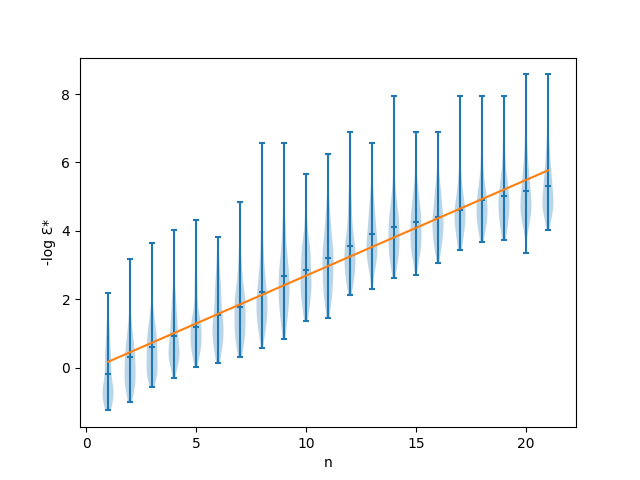
\includegraphics[width=0.9\textwidth]{errors.png}
\caption{violin plot of $\log\varepsilon^*(e, \alpha n)$ of different samples ($e$) per $n$}
\end{figure}

trend of plot shows us that the logarithmic error changes linearly by changing $n$

which can be interpreted as

\begin{equation} \log\varepsilon^*(e, \alpha n_0) \approx \alpha c_1 + c_2 \quad |~ c_1 < 0 
\end{equation}

although this simulation doesn't exactly show the existence of an stronger condition for error convergence, (as it's for a little range of small $n$s) it may be a clue for that.

UPDATE: It's proved that for an specific set of gates, the logarithmic error is a linear function of $n$ \cite{harrow}.

\begin{thebibliography}{9}
%\bibitem{shnir}
%Magnetic Monopoles
%  \url{https://link.springer.com/content/pdf/bbm%3A978-3-540-29082-7%2F1.pdf}
  
\bibitem{hamada}
\href{https://www.tamagawa.jp/research/quantum/bulletin/pdf/Tamagawa.Vol.5-5.pdf}{Hamada, M. (2015). On Parameterizations of Rotations. Tamagawa University Quantum ICT Research Institute bulletin, 5(1), 25-28.}
 
%\bibitem{biedernharn}
%Angular Momentum in Quantum Physics

\bibitem{horn}
Horn, R. A., \& Johnson, C. R. (2012). Matrix analysis. Cambridge university press.

% https://qudev.phys.ethz.ch/content/courses/QSIT07/presentations/Schmassmann.pdf

\bibitem{dawson}
\href{https://arxiv.org/pdf/quant-ph/0505030.pdf}{Dawson, C. M., \& Nielsen, M. A. (2005). The solovay-kitaev algorithm. arXiv preprint quant-ph/0505030.}

\bibitem{ozlos}
\href{http://home.lu.lv/~sd20008/papers/essays/Solovay-Kitaev.pdf}{Ozols, M. (2009). The solovay-kitaev theorem. Essay at University of Waterloo.}

\bibitem{harrow}
\href{https://arxiv.org/pdf/quant-ph/0111031.pdf}{Harrow, A. W., Recht, B., & Chuang, I. L. (2002). Efficient discrete approximations of quantum gates. Journal of Mathematical Physics, 43(9), 4445-4451.}

\end{thebibliography}
\end{document}

% todo 
% Can Be filled :)) https://en.wikipedia.org/wiki/Solovay%E2%80%93Kitaev_theorem 

% what is this? :)) https://arxiv.org/pdf/1203.6151.pdf